\documentclass{book}

\usepackage{feynmanslop}

\title{Fisica}
\author{Autore}
\date{\today}


\begin{document}



\begin{titlepage}

\maketitle

\epigraph{If, in some cataclysm, all of scientific knowledge were
to be destroyed, and only one sentence passed on to the next generations
of creatures, what statement would contain the most information in the
fewest words? I believe it is the \textit{atomic hypothesis} [...]
that \textit{all things are made of atoms—little particles that move
around in perpetual motion, attracting each other when they are a little
distance apart, but repelling upon being squeezed into one another.}
In that one sentence, you will see, there is an enormous amount of
information about the world, if just a little imagination and
thinking are applied.}{Richard P. Feynman,\\\textit{The Feynman Lectures on Physics}}

\vspace*{9cm}
\begin{center}
Consigliamo di consultare questa dispensa ascoltando il brano seguente:\\
\href{https://www.youtube.com/watch?v=JuSsvM8B4Jc}{\textcolor{blue}{\textit{Cornfield Chase} by Hans Zimmer (from \textit{Interstellar})}}
\end{center}

\end{titlepage}



\dominitoc %otherwise tocs won't appear
\tableofcontents


\part{Book}

% Lezione 1/2024-02-26
% - Introduzione filosofica alla fisica (di che si occupa, rapporto con la realta' e filosofia della quantificazione, metodo scientifico)
% - Quantificazione: misura ed errore di misura, stima

% Lezione 2/2024-02-28
% - Notazioni sulla quantificazione: ordine di grandezza
% (include altri argomenti, ma con un capitolo dedicato)

\chptr{Introduzione alla Fisica}

\section{Definizione e scopi della fisica}

Si possono formulare definizioni diverse riguardo la disciplina scientifica
della fisica, come la seguente:

\vspace{8pt}
\begin{tcolorbox}[colback = yellow!30, colframe = yellow!30!black, title = {Fisica}]
La fisica è lo studio quantitativo delle leggi fondamentali della natura, cioè
delle leggi che governano tutti i fenomeni naturali dell'universo.

Una legge fisica è una regolarita' della natura esprimibile in forma matematica.
\end{tcolorbox}
\vspace{5pt}

La fisica si avvale del \textbf{metodo scientifico}, secondo cui la natura deve
essere interrogata per vie sperimentali, facendosi guidare da \textbf{ipotesi} e
modelli teorici. Una particolarita' di questo metodo è la capacita' di isolare
un certo fenomeno che si intende studiare, tralasciando (si usera' spesso il
termine \textit{trascurare}) certi aspetti ritenuti non rilevanti in modo da
scoprire quelle regolarita' dalle quali potrebbe essere dedotta una certa'
relazione matematica.

Il ruolo della matematica è di fornire un linguaggio formale per descrivere
quantitativamente i fenomeni osservati e costruire modelli utili alla loro
trattazione.



\section{Grandezze fisiche}
La fisica è una scienza quantitativa, ovvero essa si occupa di caratteristiche
e proprieta' del mondo che possono essere misurate e quantificate: le cosiddette
grandezze fisiche. Esempi di grandezze fisiche sono la lunghezza, la massa, la
temperatura, la durata temporale e cosi' via.

\vspace{8pt}
\begin{tcolorbox}[colback = yellow!30, colframe = yellow!30!black, title = {Grandezza fisica}]
Una grandezza fisica è una caratteristica di un oggetto o di un fenomeno che puo'
essere misurata in termini quantitativi (oltre che oggettivi, ovvero indipendentemente
dalle sensazioni personali degli individui).
\end{tcolorbox}
\vspace{5pt}

È implicito, intuitivamente, il concetto di \textbf{misura}. Misurare una grandezza
fisica significa confrontarla con una grandezza ``campione'', detta \textbf{unita'
di misura}, e stabilire quante volte l'unita' di misura è contenuta nella
grandezza data. Il valore numerico ottenuto è la misura della grandezza e deve
essere sempre accompagnato dall'unita' di misura.
In altre parole, la \textbf{misura} non è altro che un \textit{rapporto} tra la
grandezza che si intende misurare e la grandezza campione scelta convenzionalmente
per tale scopo.

Mostriamo un esempio: supponiamo di voler misurare la lunghezza di qualsiasi cosa
in ``chiavette USB'' (si potrebbe argomentare circa quale chiavetta si stia
impiegando e quale posizione la chiavetta debba assumere durante la misura.
Supponiamo qui che la chiavetta sia posta in verticale, senza perderci in ulteriori
dettagli). Decidiamo poi di misurare l'altezza di una porta—anche qui, non
specifichiamo quale porta—utilizzando l'unita' appena scelta. Supponiamo quindi
di aver registrato il seguente dato:
\[ H = 20 \text{ chiavette USB} \]
Notare come siano stati specificati:
\begin{itemize}
    \item Un nome per l'oggetto che si intendeva misurare, $H$, ovvero l'altezza
    della porta.
    \item Il valore numerico individuato, 20.
    \item Una affermazione per legare il nome e il dato, = (``corrisponde a'', ``è
    uguale a'')—caratteristica che peraltro si trova anche nei linguaggi di
    programmazione.
    \item L'unita' di misura, chiavette USB.
\end{itemize}
Tuttavia, tale misurazione non è stata affatto ``sincera'': non vi è la
garanzia del fatto che il valore registrato sia esatto. La prossima sezione
trattera' questo problema, ovvero quello dell'\textit{incertezza}.


\section{Incertezza}
Idealmente, si vorrebbe impiegare, grazie alle misure, numeri puntuali ed esatti.
In altre parole, dei numeri con una precisione indefinita, aventi un numero
illimitato di cifre decimali e non.

Ma quando si effettua una misura di una grandezza, il risultato ottenuto è noto solo
con una certa precisione. Riprendendo l'esempio della chiavetta USB, è impossible
misurare con certezza tutte le lunghezze, in quanto non multipli esatti della
chiavetta stessa: ci sara' sempre un certo margine di ``un pezzo di chiavetta'',
minore dell'unita' prescelta. Ma al di sotto di quella unita' non è possibile
fornire alcuna garanzia sulla puntualita' del dato. In altre parole, la
\textit{sensibilità}\footnote{La più piccola variazione della grandezza che lo
strumento è in grado di rilevare.} dello strumento è uno dei limiti alla precisione
della misura.

\vspace{8pt}
\begin{tcolorbox}[colback = yellow!30, colframe = yellow!30!black, title = {Cifre significative del risultato di una misura}]
Le cifre significative del risultato di una misura sono le cifre note
con certezza e la prima cifra incerta. In altre parole, esse sono le cifre che si
possono controllare con lo strumento impiegato nella misura.
\end{tcolorbox}
\vspace{5pt}

Ad esempio, il valore corrispondente alla lunghezza di una barca $L = 10,5$ m
possiede tre cifre significative, che non equivale a $10,50$ m. Il secondo dato,
infatti, dichiara che la misurazione è stata possibile controllando le cifre
fino al centimetro. $L = 0,002$ possiede solo una cifra significativa, perché
in genere si ignorano gli zeri a sinistra della prima cifra significativa diversa
da zero. Possono essere ambigui valori come $L = 2500 \text{ m}$: quali zeri sono
cifre significative? Come vedremo tra poco, è utile esprimere questi valori in
notazione scientifica per eliminare ambiguità.

Vi potrebbero anche essere errori dovuti a imprecisioni introdotte nell'utilizzo
degli strumenti di misura. Questo errore deve tuttavia essere quantificato ed ogni
misura ne è affetta (comprese quelle che non la riportano).

\vspace{8pt}
\begin{tcolorbox}[colback = yellow!30, colframe = yellow!30!black, title = {Risultato della misura di una grandezza}]
Il risultato della misura di una grandezza è sempre un'approssimazione
accompagnata da una certa incertezza, ovvero un \textbf{valore attendibile}
e un \textbf{errore assoluto} (o semplicemente \textit{incertezza}).
\[ x = \overline{x} \pm e_x  \]
\end{tcolorbox}
\vspace{5pt}

Questo risultato non è quindi altro che un intervallo in cui il valore reale
della misura si trova. Ci limiteremo agli errori relativi a singole misure,
nelle quali $x$ corrisponde al valore misurato e $e_x$ la sensibilità dello
strumento. Di conseguenza, possiamo ora correggere il risultato della misura
effettuata in chiavette USB:
\[ H = (20 \pm 1) \text{ chiavette USB} \]

\section{Notazione scientifica e ordini di grandezza}
Unità di misura come il metro e il kologrammo sono comode nella vita di tutti i
giorni, ma rappresentano quantità enormi su scala atomica e subatomica e quantità
minuscole su scala astronomica e cosmica. Conseguenza di ciò è che alcune misure
possono essere espresse da numeri ``scomodi''. Considerando solo valori attendibili,
la massa dell'atomo di idrogeno è circa
\[ m_H = 0,000 000 000 000 000 000 000 000 001 67 \text{ kg} \]
mentre la massa della Terra è
\[ m_T = 5 970 000 000 000 000 000 000 000 \text{ kg} \]
È pressoché evidente il motivo di tale scomodità: la notazione è di difficile
trattazione. Viene dunque in aiuto la \textbf{notazione scientifica}, ovvero una
notazione numerica che permette di contrarre rappresentazioni estese impiegando
potenze di 10. Nella notazione scientifica, ogni numero è scritto come prodotto
di due fattori:
\begin{itemize}
    \item Un numero decimale $x:x\in R, 1\leq x < 10$\footnote{In realtà, questa notazione corrisponde alla variante ``ingegneristica''. Esiste anche una notazione che prevede che il valore espresso $x$ sia $0\leq x < 1$.}.
    \item Una potenza di 10, con esponente intero.
\end{itemize}
Pertanto, le misure precedenti si possono esprimere in notazione scientifica come
segue:
\[ m_H = 1,67 \cdot 10^{-27} \text{ kg} \]
\[ m_T = 5,97 \cdot 10^{24} \text{ kg}\]
Notare come la notazione sia in grado di eliminare ambiguità sul numero di cifre
significative: ora sappiamo che la massa della Terra è stata calcolata fino a
tre cifre significative e non 25.

Non sempre è necessario calcolare esattamente il valore di una certa grandezza.
Talvolta basta averne solo un'idea approssimata. Supponiamo, ad esempio, che sia
sufficiente sapere se una certa massa vale all'incirca 1 grammo oppure 1
ettogrammo. In questo caso, possiamo accontentarci di stimare il valore della
massa con un'accuratezza di un fattore 10, cioè di calcolare il suo ordine di
grandezza.

\vspace{8pt}
\begin{tcolorbox}[colback = yellow!30, colframe = yellow!30!black, title = {Ordine di grandezza}]
L'ordine di grandezza di un numero è la potenza di 10 più vicina a quel numero.
\end{tcolorbox}
\vspace{5pt}

Per determinare l'ordine di grandezza di un numero occorre quindi esprimerlo in
notazione scientifica—prodotto di un numero decimale compreso tra 1 e 10 e di
una potenza di 10—e poi approssimare il valore alla potenza di 10 più vicina.
In particolare:
\begin{itemize}
    \item Se il numero decimale è minore di 5, si mantiene l'esponente della
    potenza. Ad esempio:
    \[ 3,6 \cdot 10^2 \to \text{ Ordine di grandezza } 10^2 \]
    \[ 4,2 \cdot 10^{-3} \to \text{ Ordine di grandezza } 10^{-3} \]

    \item Se il numero decimale è maggiore di 5, si somma +1 all'esponente della
    potenza. Ad esempio:
    \[ 9 \cdot 10^2 \approx 10 \cdot 10^2 \to \text{ Ordine di grandezza } 10^3 \]
    \[ 8,1 \cdot 10^{-12} \approx 10 \cdot 10^{-12} \to \text{ Ordine di grandezza } 10^{-11} \]
\end{itemize}


Sono stati definiti dei prefissi stadard per certi ordini di grandezza notevoli,
cioè quelli che, escludendo la potenza nulla, rappresentano multipli di tre.
Utilizzando questi prefissi, di fianco all'unità di misura adottata, si contrae
ancora di più la notazione scientifica, sottointendendo un certo ordine di
grandezza.

\marginpar{
    \footnotesize
    %\hspace*{-0.5cm}
    \begin{tabular}{c|c|c}
        Potenza   & Simbolo & Prefisso\\
        \hline
        $10^{12}$  & T       & Tera\\
        $10^{9}$   & G       & Giga\\
        $10^{6}$   & M       & Mega\\
        $10^{3}$   & k       & kilo\\
        $10^{-3}$  & m       & milli\\
        $10^{-6}$  & $\mu$   & micro\\
        $10^{-9}$  & n       & nano\\
        $10^{-12}$ & p       & pico\\
    \end{tabular}
}
% Lezione 2/2024-02-28
% - Introduzione alla descrizione quantitativa del moto (cinematica?)
% - cinematica del punto materiale da una a piu' dimensioni: moto rettilineo uniforme, piano cartesiano
% - equazioni del moto, con notazione vettoriale
% Esercitarsi su: moto rettilineo uniforme, vettori e trigonometria, sistemi di riferimento cartesiani e algebra sul piano cartesiano


\chptr{Descrizione del moto}

\section{Introduzione al moto del punto materiale}
Un corpo è in moto quando la sua posizione cambia nel tempo. Nel descrivere il
moto, si introdurrà la seguente semplificazione: gli oggetti in moto saranno
trattati come \textit{punti materiali}, ovvero concentrati in un punto
adimensionale. Il modello del punto materiale è un buon punto di partenza per
comprendere bene il fenomeno del moto (cominciare dal quadro attuale, ovvero
quello della relatività ristretta, sarebbe interessante ma ostico). In particolare,
\textit{le dimensioni dell'oggetto del quale si intende studiare il moto saranno
considerate trascurabili rispetto a quelle dell'ambiente circostante}.

\subsection{Sistemi di riferimento}
Abbiamo detto che il moto è caratterizzato da un cambiamento di posizione. Il primo
passo nella descrizione del moto di un corpo consiste quindi nello stabilire il
modello da adottare per catturare il concetto di \textbf{posizione}. Sappiamo già
che i modelli della fisica si basano sul linguaggio matematico; il modello più
naturale che si possa adottare è dunque un sistema di assi cartesiani. Da qui, la
posizione del corpo può essere specificata mediante coordinate. Una speciale
coordinata è il tempo.

La scelta del sistema di riferimento di assi cartesiani è del tutto arbitraria,
ma una volta fissata è necessario essere coerenti con essa.


\section{Moto rettilineo uniforme}

\begin{marginfigure}
    \centering
    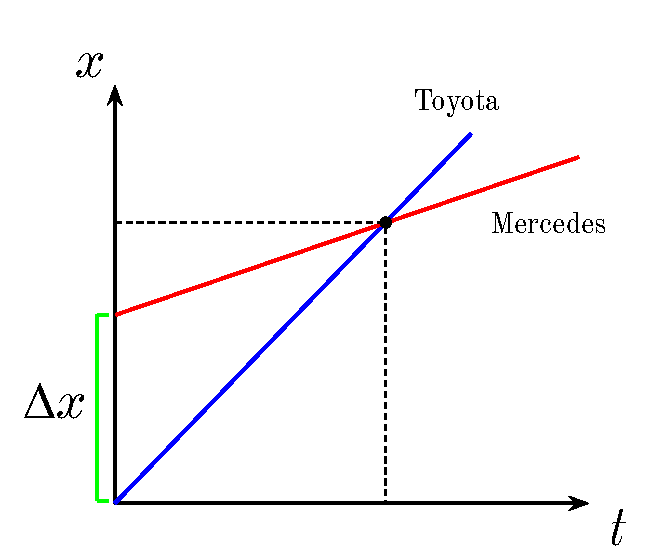
\includegraphics[width = \marginparwidth]{figures/sorpasso.pdf}
    \caption{Un caso di sorpasso}
\end{marginfigure}

\[  \]
\[ x(t) = x_i + v(t - t_i)  \]
% Lezione 3/2024-03-04
% - introduzione alla dinamica
% - prima e seconda legge
% - esercizi su moto uniformemente accelerato
% - accenni al concetto di forza e introduzione alla forza elastica con legge di hooke

% Lezione 4/2024-03-06
% - grafico orario: grafico nel quale un asse riporta lo spazio (una dimensione), mentre sull'altro il tempo
% - differenza tra SPOSTAMENTO e distanza
% - interpretazione grafica della velocità e accelerazione, con analisi di funzione

\chptr{Dinamica}
\marginpar{\minitoc}

\section{Recap}
\[ \overrightarrow{x} = \overrightarrow{x_0} + \overrightarrow{v}(t - t_0) \]
Semplificazioni in termini di variazioni, infinità.

\section{Leggi della dinamica}

Nella descrizione introduttiva del moto, non è stata analizzata alcuna causa del
fenomeno.

\subsection{La prima legge}

\vspace{8pt}
\begin{tcolorbox}[colback = red!30, colframe = red!30!black, title = {Prima legge della dinamica (legge di inerzia)}]
    Un corpo permane nel suo stato di \textit{quiete} o moto rettilineo uniforme
    finché non intervenga un \textit{agente esterno}.
\end{tcolorbox}
\vspace{5pt}

In altre parole, se nulla ``rompe le scatole'' al corpo, esso permanerà nel suo
stato di moto, naturalmente.

\vspace{8pt}
\begin{tcolorbox}[colback = yellow!30, colframe = yellow!30!black, title = {Sistema inerziale}]
    Sistema nel quale vale la prima legge della dinamica.
\end{tcolorbox}
\vspace{5pt}

\subsection{La seconda legge}
Quando l'agente esterno agisce sull'oggetto, l'effetto è un cambiamento nello
stato di moto di quell'oggetto. Ovvero, cambia la sua velocità. La variazione
della velocità nel tempo è chiamata \textbf{accelerazione}.

\[ \lim_{\Delta t \to 0} \frac{\Delta v}{\Delta t} = \frac{dv}{dt} = a \]

\vspace{8pt}
\begin{tcolorbox}[colback = red!30, colframe = red!30!black, title = {Seconda legge della dinamica}]
    \begin{align}
        \frac{|\overrightarrow{F}|}{|\overrightarrow{a}|} = \frac{F}{a} = m
    \end{align}
\end{tcolorbox}
\vspace{5pt}


Gli oggetti hanno inerzia, ovvero capacità di opporsi all'agire dell'agente
esterno. Questa capacità di opporsi è rappresentato da una quantità detta
massa (inerziale).

\subsection{Analisi dimensionale}
\[ [F] = [ma] = \left[m\cdot\frac{v}{t}\right] = \left[m\cdot\frac{l}{t^2}\right]  \]
\[ 1\text{ kg}\cdot\frac{\text{m}}{\text{s}^2} = \text{udm}\left[M\cdot\frac{L}{T^2}\right] = \text{udm}[F] = 1\text{ N} \]


\subsection{Molla e forza elastica}
\[ F \propto \Delta x \]

La forza che la molla esercita, essendo in opposizione alla direzione nella
quale la deformazione viene effettuata, corrisponde a:
\[ F_\textit{el} = -k\Delta x \]

\section{Forza agente sul moto}
Un blocco di massa $m = 10 \text{ kg}$ viaggia ad una velocità $v_i =
2 \text{ m/s}$. Una forza $F = 20 \text{ N}$ agisce sul blocco per
$T = 5 \text{ s}$. Quale velocità raggiungerà il blocco dopo $T$?.
Dopo $T$, la forza cessa di agire e il blocco viaggia a $v_f$ trovata
precedentemente. Includendo lo spazio percorso durante $T$ (e dunque il
tempo $T$), quanto tempo impiega il blocco a coprire $s_w = 2\text{ km}$
di distanza?

\begin{marginfigure}
    \centering
    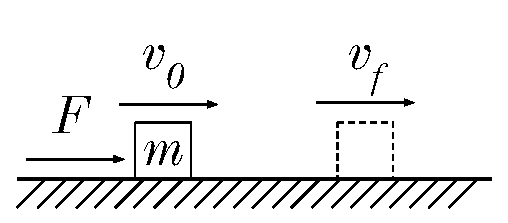
\includegraphics[width = \marginparwidth]{figures/scivola.pdf}
    \caption{Forza agente su una massa in moto}
\end{marginfigure}

Per rispondere al primo quesito, possiamo assumere un moto rettilineo
uniformemente accelerato durante l'intervallo $T$. Sappiamo che \[ a = \frac{F}{m} = \frac{dv}{dt} \]
Da cui possiamo esprimere la velocità in funzione del tempo (la velocità
iniziale la conosciamo già, ma assumiamo un tempo iniziale $t_0 = 0$):
\[ \frac{F}{m}dt = dv \to \int_{t_0}^{t}\frac{F}{m}dp = \int_{v_0}^{v}dw \to \frac{F}{m}\int_{0}^{t}dp = v - v_0 \to \frac{F}{m}t = v - v_0 \]
Dunque
\[ v(t) = v_0 + \frac{F}{m}t \]
Non ci manca che calcolare la velocità in corrispondenza di un $t_f = t_0 + \Delta t = 0 + T = T$:
\[ v(t_f) = v(T) = v_0 + \frac{F}{m}T \]

Nel secondo quesito, possiamo spezzare il problema in due parti: durante
l'azione della forza, la distanza percorsa ($s_a$) deve essere calcolata tenendo
conto del moto uniformemente accelerato, mentre nell'intervallo di tempo
successivo ($T_v$) il moto è semplicemente uniforme. Dalla seguente equazione,
possiamo ricavare $T_v$ ($T$ lo conosciamo già).
\[ s_w = s_a + s_v = s_a + v_fT_v = \int_{0}^{T}(v_0 + at)dp + v_fT_v = v_0T + \frac{1}{2}aT^2 + v_fT_v \]
Il tempo per percorrere $2\text{ km}$ è dunque:
\[ T_{2\text{ km}} = T + \frac{s_w - v_iT - \frac{F}{2m}T^2}{v_f} = T + \frac{s_w - v_iT - \frac{F}{2m}T^2}{v_i + \frac{F}{m}T} \]

\section{Lancio verso l'alto}
Si consideri la situazione mostrata in Figura \ref{lanciobasso}.
Durante la salita, l'oggetto rallenta a causa dell'accelerazione di gravità $g$.
Determiniamo la quota che l'oggetto raggiungerà.

\[ a = \frac{dv}{dt} \to dv = adt \to \int_{v_0}^{v}dw = \int_{t_0}^{t}adp \to v - v_0 = a\int_{t_0}^{t}dp \to v - v_0 = a(t - t_0) \]
Dunque
\[ v(t) = v_0 + a(t - t_0) = v_0 + at \]
Rallentando, si arriverà ad un istante $t_f$ nel quale l'oggetto avrà velocità
nulla:
\begin{marginfigure}
    \centering
    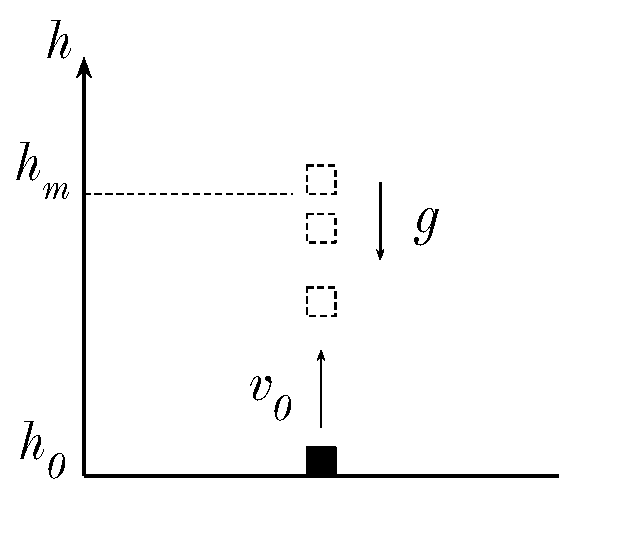
\includegraphics[width = \marginparwidth]{figures/greve.pdf}
    \caption{Lancio di un oggetto verso l'alto}
    \label{lanciobasso}
\end{marginfigure}
\[ v(t_f) = 0 \to v_0 + at_f = 0 \]
Non disponiamo tuttavia del tempo, ma possiamo avvalerci della legge oraria
che descrive la distanza percorsa:
\[ v(t) = \frac{dh}{dt} \to \int_{h_0}^{h}dk = \int_{t_0}^{t}v(t)dp \to h - h_0 = \int_{t_0}^{t}(v_0 + ap)dp \]
\[ h - h_0 = v_0\int_{t_0}^{t}dp + a\int_{t_0}^{t}pdp \to h - h_0 = v_0t + \frac12 at^2 \]
Da cui:
\[ h(t) = h_0 + v_0t + \frac12 at^2 = v_0t + \frac12 at^2 \]
Abbiamo quindi ottenuto la quota in funzione del tempo, che possiamo ricavare
dall'equazione $v_0 + at_f = 0 \to t_f = -\frac{v_0}{a}$.
\[ h(t_f) = v_0t_f + \frac12 at_{f}^2 =  -\frac{v_0^2}{a} + \frac{1}{2}a\frac{v_0^2}{a^2} = -\frac{v_0^2}{a} + \frac{v_0^2}{2a} = -\frac{v_0^2}{2a} \]
Sapendo che $a = -|g|$, la quota massima $h_m$ raggiunta è:
\[ h_m = \frac{v_0^2}{2|g|} \]

%%%%%%%%%%%%%%%%%%%%%%%%%%%%%%%%%%%%%%%%%%%%%%%%%%%%%%%%%%%%%%%%%

\subsection*{Spostamento}
\[ \Delta\overrightarrow{s} = \overrightarrow{s}_f - \overrightarrow{s}_i \]


\subsection{La terza legge}
\vspace{8pt}
\begin{tcolorbox}[colback = red!30, colframe = red!30!black, title = {Terza legge della dinamica}]

\end{tcolorbox}
\vspace{5pt}



\vspace{8pt}
\begin{tcolorbox}[colback = red!30, colframe = red!30!black, title = {Accelerazione centripeta nel moto circolare uniforme}]
\begin{align}
    a = \frac{v^2}{r} = \omega^2 r
\end{align}
\end{tcolorbox}
\vspace{5pt}


\part{Lezioni}

%\chptr{Test}

\section{Thermodynamics}
\marginpar{\epigraph{Il problema non è \textit{dove}..., nemmeno \textit{quando}..., solo il \textit{come} importa.}{Anonimo}}
\marginpar{\minitoc}


Lorem ipsum dolor sit amet, consectetuer adipiscing elit. Etiam lobortis facilisis
sem. Nullam nec mi et neque pharetra sollicitudin. Praesent imperdiet mi nec
ante. Donec ullamcorper, felis non sodales commodo, lectus velit ultrices augue,
a dignissim nibh lectus placerat pede. Vivamus nunc nunc, molestie ut, ultricies
vel, semper in, velit. Ut porttitor. Praesent in sapien. Lorem ipsum dolor sit
amet, consectetuer adipiscing elit. Duis fringilla tristique neque. Sed interdum
libero ut metus. 


\begin{marginfigure}
  \centering
  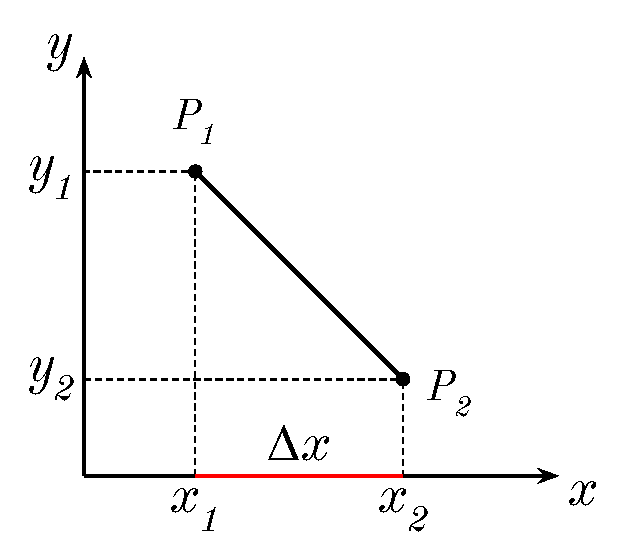
\includegraphics[width = \marginparwidth]{figures/moto.pdf}
  \caption{VS Code logo, with some caption below}
\end{marginfigure}

\vspace*{0.2cm}
\begin{tcolorbox}[colback = yellow!30, colframe = yellow!30!black, title = {Some equations}]
Brief description.
  \begin{align}
  \int_{-\infty}^{+\infty}f(x)dx = 1\label{integrale}\\
  \sum_{i = 0}^{+\infty} \frac{1}{2^i} = 2\label{sommatoria}
\end{align}

\end{tcolorbox}

Lorem ipsum dolor sit amet, consectetuer adipiscing elit. Etiam lobortis facilisis
sem. Nullam nec mi et neque pharetra sollicitudin. Praesent imperdiet mi nec
ante. Donec ullamcorper, felis non sodales commodo, lectus velit ultrices augue,
a dignissim nibh lectus placerat pede. Vivamus nunc nunc, molestie ut, ultricies
vel, semper in, velit. Ut porttitor. Praesent in sapien. Lorem ipsum dolor sit
amet, consectetuer adipiscing elit. Duis fringilla tristique neque. Sed interdum
libero ut metus. 

\subsection{First law of Thermodynamics}
Lorem ipsum dolor sit amet, consectetuer adipiscing elit. Etiam lobortis facilisis
sem. Nullam nec mi et neque pharetra sollicitudin. Praesent imperdiet mi nec
ante. Donec ullamcorper, felis non sodales commodo, lectus velit ultrices augue,
a dignissim nibh lectus placerat pede. Vivamus nunc nunc, molestie ut, ultricies
vel, semper in, velit. Ut porttitor. Praesent in sapien. Lorem ipsum dolor sit
amet, consectetuer adipiscing elit. Duis fringilla tristique neque. Sed interdum
libero ut metus. Equazione \ref{integrale} e \ref{sommatoria}.

\section{Cinematics}
Lorem ipsum dolor sit amet, consectetuer adipiscing elit. Etiam lobortis facilisis
sem. Nullam nec mi et neque pharetra sollicitudin. Praesent imperdiet mi nec
ante. Donec ullamcorper, felis non sodales commodo, lectus velit ultrices augue,
a dignissim nibh lectus placerat pede. Vivamus nunc nunc, molestie ut, ultricies
vel, semper in, velit. Ut porttitor. Praesent in sapien. Lorem ipsum dolor sit
amet, consectetuer adipiscing elit. Duis fringilla tristique neque. Sed interdum
libero ut metus.

\marginpar{
  \begin{tabular}{c|c}
    Heading & Heading\\
    \hline
    Hello & Hello
  \end{tabular}
}

\section{Other section}
\section{More sections}
\section{More}
\section{Another one please}
\section*{Unnnumbered section}
\section{More}
\section{Another one please}
\section{More}
\section{Another one please, but way longer such that it does not fit the margin}

\chptr{Lezione 2024-02-26}
\section*{Riassunto}
\begin{itemize}
    \item Dinamica: dinamica del punto materiale (3 leggi dinamica)
    \item Meccanica: quantita' conservative (energia ecc)
    \item Termodinamica dei gas
    \item Entropia/probabilita'/senso del tempo
    \item Elettricita': Coulomb
    \item Magnetismo
\end{itemize}

\chptr{Test}

\section{Thermodynamics}
\marginpar{\epigraph{Il problema non è \textit{dove}..., nemmeno \textit{quando}..., solo il \textit{come} importa.}{Anonimo}}
\marginpar{\minitoc}


Lorem ipsum dolor sit amet, consectetuer adipiscing elit. Etiam lobortis facilisis
sem. Nullam nec mi et neque pharetra sollicitudin. Praesent imperdiet mi nec
ante. Donec ullamcorper, felis non sodales commodo, lectus velit ultrices augue,
a dignissim nibh lectus placerat pede. Vivamus nunc nunc, molestie ut, ultricies
vel, semper in, velit. Ut porttitor. Praesent in sapien. Lorem ipsum dolor sit
amet, consectetuer adipiscing elit. Duis fringilla tristique neque. Sed interdum
libero ut metus. 


\begin{marginfigure}
  \centering
  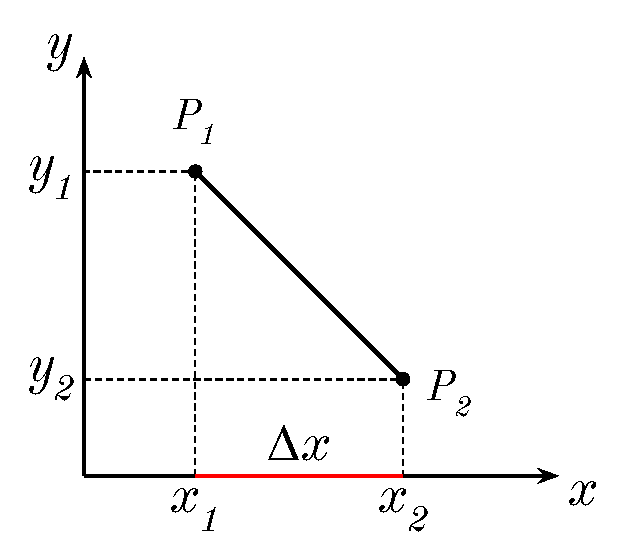
\includegraphics[width = \marginparwidth]{figures/moto.pdf}
  \caption{VS Code logo, with some caption below}
\end{marginfigure}

\vspace*{0.2cm}
\begin{tcolorbox}[colback = yellow!30, colframe = yellow!30!black, title = {Some equations}]
Brief description.
  \begin{align}
  \int_{-\infty}^{+\infty}f(x)dx = 1\label{integrale}\\
  \sum_{i = 0}^{+\infty} \frac{1}{2^i} = 2\label{sommatoria}
\end{align}

\end{tcolorbox}

Lorem ipsum dolor sit amet, consectetuer adipiscing elit. Etiam lobortis facilisis
sem. Nullam nec mi et neque pharetra sollicitudin. Praesent imperdiet mi nec
ante. Donec ullamcorper, felis non sodales commodo, lectus velit ultrices augue,
a dignissim nibh lectus placerat pede. Vivamus nunc nunc, molestie ut, ultricies
vel, semper in, velit. Ut porttitor. Praesent in sapien. Lorem ipsum dolor sit
amet, consectetuer adipiscing elit. Duis fringilla tristique neque. Sed interdum
libero ut metus. 

\subsection{First law of Thermodynamics}
Lorem ipsum dolor sit amet, consectetuer adipiscing elit. Etiam lobortis facilisis
sem. Nullam nec mi et neque pharetra sollicitudin. Praesent imperdiet mi nec
ante. Donec ullamcorper, felis non sodales commodo, lectus velit ultrices augue,
a dignissim nibh lectus placerat pede. Vivamus nunc nunc, molestie ut, ultricies
vel, semper in, velit. Ut porttitor. Praesent in sapien. Lorem ipsum dolor sit
amet, consectetuer adipiscing elit. Duis fringilla tristique neque. Sed interdum
libero ut metus. Equazione \ref{integrale} e \ref{sommatoria}.

\section{Cinematics}
Lorem ipsum dolor sit amet, consectetuer adipiscing elit. Etiam lobortis facilisis
sem. Nullam nec mi et neque pharetra sollicitudin. Praesent imperdiet mi nec
ante. Donec ullamcorper, felis non sodales commodo, lectus velit ultrices augue,
a dignissim nibh lectus placerat pede. Vivamus nunc nunc, molestie ut, ultricies
vel, semper in, velit. Ut porttitor. Praesent in sapien. Lorem ipsum dolor sit
amet, consectetuer adipiscing elit. Duis fringilla tristique neque. Sed interdum
libero ut metus.

\marginpar{
  \begin{tabular}{c|c}
    Heading & Heading\\
    \hline
    Hello & Hello
  \end{tabular}
}

\section{Other section}
\section{More sections}
\section{More}
\section{Another one please}
\section*{Unnnumbered section}
\section{More}
\section{Another one please}
\section{More}
\section{Another one please, but way longer such that it does not fit the margin}

\setcounter{chapter}{0}

\part{Esercitazioni}


\end{document}